\section{Theory of relaxation of electromagnetic filed. Heisenberg--Langevin method}

\subsection{In previous series}

We have discussed:
\begin{enumerate}
	\item Two-level system (e.g. atom) and one mode field. Result: Rabi oscillations.
	\item Two-level system and continuum of modes (e.g. cavity). Result: spontaneous emission.
	\item One-mode field in the cavity and continuum of modes. Result: let's find out!
\end{enumerate}

\begin{figure}[h!]
	\centering
	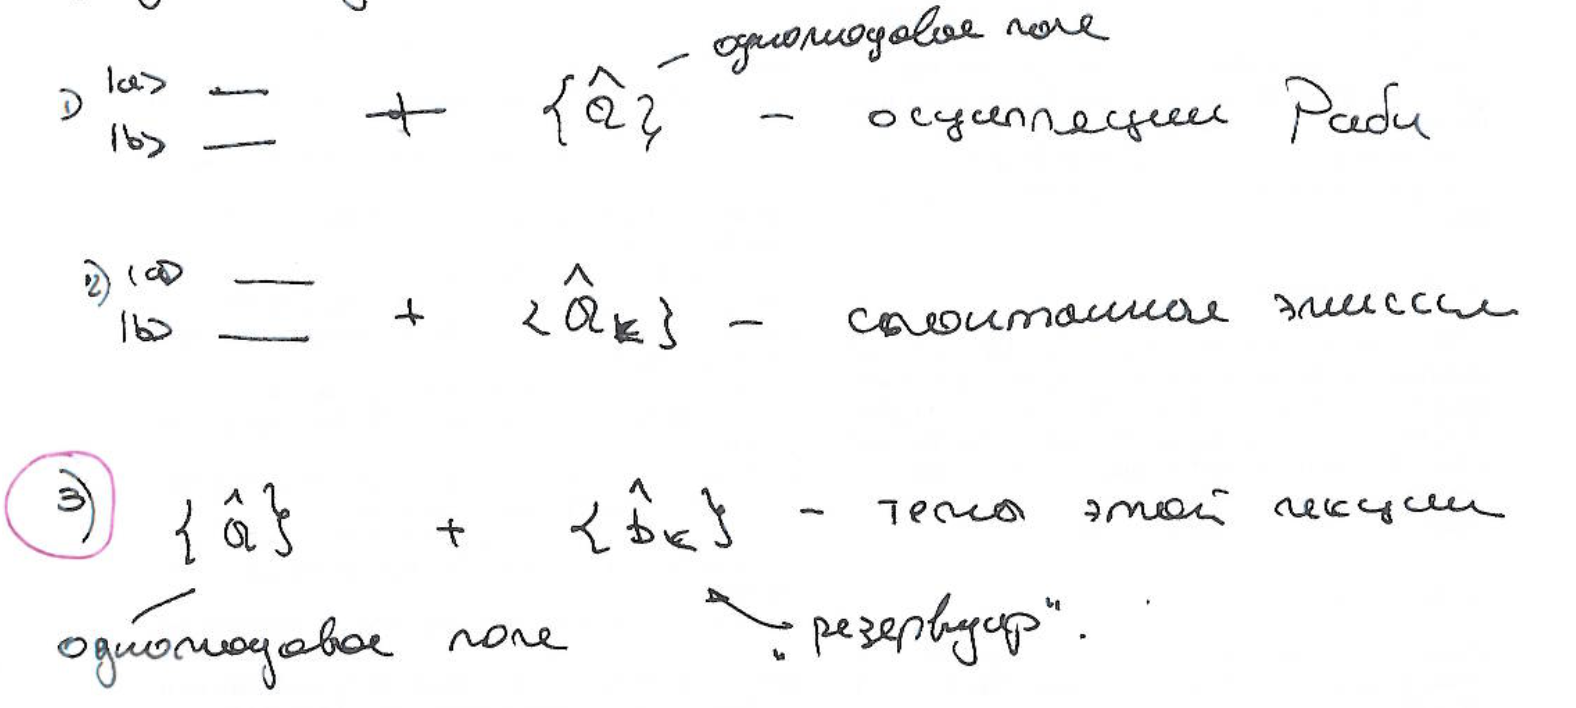
\includegraphics[width=0.8\linewidth]{fig/L9/fig1}
	\caption{Different possible cases for analytical consideration.}
	\label{fig:fig11}
\end{figure}

\subsection{the Heisenberg--Langevin equation}

We are interested in dynamics of $\hat{b}(t)$ and $\hat{a}(t)$ in thermodynamics equilibrium at the temperature $T$. We consider modes which are fluctuate independently
\begin{eqnarray}
	\left \langle \hat{b}^{\dagger}_{\kv} (0) \hat{b}_{\kv'} (0) \right \rangle &=& \bar{n}_{\kv} \delta_{\vec{k}\vec{k}'}, \\
	\av{\hat{b}_{\kv}(0)} = \av{\hat{b}^{\dagger}_{\kv}(0)} &=& 0,\\
	\av{\hat{b}_{\kv} (0) \hat{b}^{\dagger}_{\kv'} (0) } &=& (\bar{n}_{\kv}+1) \delta_{\vec{k}\vec{k}'}, \\
	\av{\hat{b}_{\kv} (0) \hat{b}_{\kv'} (0) } = \av{\hat{b}^{\dagger}_{\kv} (0) \hat{b}^{\dagger}_{\kv'} (0) } &=& 0.
\end{eqnarray}
Here and  hereinafter the angle brakes represent the reservoir averages $\av{\dots} \equiv \av{\dots}_{\text{R}}$.

As the wave function is unknown we use the density matrix approach. Density matrix and distribution function in thermodynamics equilibrium is given by
\begin{equation}
	\rho_R = \Pi \left( 1 - e^{- \frac{\hbar \omega_{\vec{k}}}{kT}} \right) e^{- \frac{\hbar \omega_{\vec{k}} \hat{b}_{\kv}^{\dagger} \hat{b}_{\kv}}{kT}}, \qquad \bar{n}_{\kv}  = \frac{1}{e^{\frac{\hbar \omega_{\vec{k}}}{kT}} - 1}.
\end{equation}
The Hamiltonian of the system can be written as
\begin{equation}
	\hat{\mathcal{H}} = \underbrace{\hbar \omega \hat{a}^{\dagger} \hat{a}}_{\text{resonator}} + \underbrace{\sum_{\kv} \hbar \omega_{\kv} \hat{b}^{\dagger}_{\kv} \hat{b}_{\kv}}_{\text{cavity}} + \underbrace{\sum_{\kv} \hbar  \left( g_{\kv} \hat{b}_{\kv}^{\dagger} \hat{a}_{\kv} + g^*_{\kv} \hat{a}_{\kv}^{\dagger} \hat{b}_{\kv}  \right)}_{\hat{\mathcal{H}}_{\text{int}}}.
\end{equation}
The  explicit form of $g_{\kv}$ is strongly depend on exact system. However we know the asymptotic behavior --- if the resonator is ideal then $g_{\kv} = 0$.

Time evolution is defined by
\begin{equation}
	\hat{\dot{a}}(t) = \frac{i}{\hbar} \left[ \hat{\mathcal{H}}, \hat{a}  \right], \qquad  	\hat{\dot{b}}(t) = \frac{i}{\hbar} \left[ \hat{\mathcal{H}}, \hat{b}  \right],
\end{equation}
which gives
\begin{numcases}{}
		\hat{\dot{a}}(t) = -i \omega \hat{a}(t) - i \sum_{\kv} g_{\kv}^* \hat{b}_{\kv}(t), \label{eq:a_dyn}\\
		\hat{\dot{b}}_{\kv}(t) = -i \omega_{\kv} \hat{b}_{\kv}(t) - i  g_{\kv} \hat{a}(t),
		\label{eq:b_dyn}
\end{numcases}
Important to notice that it is sensible to consider only the mean values of operators.

Now let us solve this system. it is easy to verify that the solution of  \eqref{eq:b_dyn}  is
\begin{equation}
	\hat{b}_{\kv}(t) = \underbrace{\hat{b}_{\kv}(0) e^{-i\omega_{\kv} t}}_{\text{reservoir modes evolution}} - \underbrace{i g_{\kv} \int \limits_0^{t} d\tau \hat{a}(\tau) e^{-i\omega_{\kv}(t - \tau)}}_{\text{interaction between reservoir and oscillator}}
\end{equation}
then we substitute this result in \eqref{eq:a_dyn} and obtain
\begin{equation}
	\hat{\dot{a}}(t) = - i \omega \hat{a}(t) - \hat{f}_a(t) + \sum_{\kv} \left| g_{\kv} \right|^2 \int \limits_0^td\tau \hat{a}(\tau) e^{-i\omega_{\kv}(t - \tau)},
\end{equation}
where
\begin{equation}
	\hat{f}_a(t) \myeq i \sum_{\kv} g_{\kv}^* \hat{b}_{\kv}(0) e^{-i\omega_{\kv} t}
\end{equation}
is a stochastic operator as the number of photons in a particular time moment is undefined. After that we introduce
\begin{equation}
	\hat{\tilde{a}}(t) \myeq \hat{a}(t) e^{i \omega t}, \qquad \hat{F}_{\tilde{a}} (t) = \hat{f}_a(t) e^{i \omega t}
\end{equation}
and obtain \textit{a stochastic integro-differential equation}
\begin{equation}
	\hat{\dot{\tilde{a}}}(t) = \sum_{\kv} \left| g_{\kv} \right|^2 \int \limits_0^t d\tau \hat{\tilde{a}} e^{i(\omega-\omega_{\kv})(t - \tau)} + \hat{F}_{\tilde{a}} (t).
	\label{eq:st_int_dif}
\end{equation}
which is quite hard to solve, unless one was educated in the USSR.

To find a solution of \eqref{eq:st_int_dif} we, first of all, make transition from sum to the integral
\begin{equation}
	\sum_{\kv} \left| g_{\kv} \right|^2 \quad \to \quad \frac{V}{\pi^2 c^3} \int \limits_0^{\infty} d \omega_{\kv} \omega_{\kv}^2 \left| g_{\omega_{\kv}} \right|^2.
\end{equation}
Now let us consider only the integral in \eqref{eq:st_int_dif} which becomes
\begin{multline}
	\frac{V}{\pi^2 c^3} \int \limits_0^{\infty} d \omega_{\kv} \omega_{\kv}^2 \left| g_{\omega_{\kv}} \right|^2 \int \limits_0^t d\tau \hat{\tilde{a}}(\tau)e^{i(\omega - \omega_{\kv})(t - \tau)} = \\ =\Bigg/ \omega_{\kv}^2 \left| g_{\omega_{\kv}} \right|^2 \text{ is a slow function} \Bigg/
	\approx \frac{V}{\pi^2 c^3} \int \limits_0^t d \tau \hat{\tilde{a}}(\tau) \cdot \omega_{\kv}^2 \left| g_{\omega_{\kv}} \right|^2 \cdot  \underbrace{\int \limits_0^{\infty} d \omega_{\kv} e^{i(\omega - \omega_{\kv})(t - \tau)}}_{\hookrightarrow\approx 2\pi \delta(t - \tau)} =\\= \frac{V}{\pi^2 c^3} \omega_{\kv}^2 \cdot 2 \pi \left| g_{\omega_{\kv}} \right|^2 \underbrace{\int \limits_0^t d\tau \hat{\tilde{a}}(\tau) \delta(t - \tau)}_{\half \hat{\tilde{a}}(t)}  =\frac{\Gamma}{2}\hat{\tilde{a}}(t),
\end{multline}
where we defined a relaxation constant $\Gamma$ and density of states $D$:
\begin{equation}
	\Gamma \myeq D(\omega_{\kv}) \cdot 2 \pi \left| g_{\omega_{\kv}} \right|^2  , \qquad D(\omega_{\kv}) = \frac{V \omega_{\kv}^2}{\pi^2 c^3} = \int d^3 r \rho(\vec{r}, \omega_{\kv}).
\end{equation}
So finally here is \textit{the Heisenberg--Langevin equation}:
\begin{equation}
	\boxed{\hat{\dot{\tilde{a}}}(t) = - \frac{\Gamma}{2} \hat{\tilde{a}}(t) + \hat{F}_{\tilde{a}} (t). }
	\label{eq:HLeq}
\end{equation}

\textit{Remark:} we could obtain the same result if we would have considered the dynamics of atom's operator $\hat{\dot{\sigma}}_z(t)$.

\begin{testexample}[Connection between dissipation and fluctuation]
	Let us put $\hat{F}_{\tilde{a}} (t) = 0$. It means that $\hat{\tilde{a}}(t) = \hat{\tilde{a}}(0) e^{- \frac{\Gamma}{2} t}$ which leads to
	\begin{equation}
		\left[ \hat{\tilde{a}}(t), \hat{\tilde{a}}^{\dagger}(t) \right] = e^{- \Gamma t} \neq 1.
		\label{eq:example}
	\end{equation}
	That is nonsense! It couldn’t be, so we can not just put the stochastic term to zero. \textit{If there is a dissipation then there have to be fluctuation in the system.}
\end{testexample}




\begin{hw}[Deadline: 29th of December]
	\addcontentsline{toc}{subsubsection}{Homework}

	\begin{enumerate}
		\item (4 pts) Consider two interacting cavities  described by the  Hamiltonian:
		
		$$
		H=\hbar \omega a^{+}a+\hbar\omega b^{+}b+\hbar g(a^{+}b+b^{+}a)
		$$
		 Initially  there were  $N_{a}$ and $N_{b}$ photons in each resonator. Please, describe how the number of photon will change in time in each resonator.
		
		 {\it Hint}:  use the equation of operator motion to calculate $\hat n _a$ and $\hat n _b$
	
	\end{enumerate}
\end{hw}

\subsection{Properties of the stochastic operator}

Let us find out properties of the stochastic operator $\hat{F}_a(t)$. The mean values are
\begin{equation}
	\av{\hat{F}_a(t)} = \av{\hat{F}_a^{\dagger}(t)} = 0.
\end{equation}
Now let us find the correlator
\begin{multline}
	\av{\hat{F}_a^{\dagger}(t) \hat{F}_a(t')} = \sum_{\kv \kv'} g^*_{\kv} g_{\kv'} \underbrace{\cdot \av{\hat{b}_{\kv}^{\dagger}(0) \hat{b}_{\kv}(0)} \cdot }_{\overset{\hookrightarrow=\bar{n}_{\kv} \delta_{\vec{k}\vec{k}'}}{\text{av. num. of ph. in } \kv}} e^{i(\omega_{\kv} - \omega)t - i(\omega_{\kv'} - \omega)t'} = \\
	= \sum_{\kv} \left| g_{\kv}\right|^2 \bar{n}_{\kv} e^{i (\omega_{\kv} - \omega)(t - t')} = \int \limits_0^{\infty} d \omega_{\kv} D(\omega_{\kv}) \left| g_{\kv}\right|^2 \bar{n}_{\kv} (\omega_{\kv}) e^{i (\omega_{\kv} - \omega)(t - t')} \approx \\ \approx \underbrace{D(\omega_{\kv}) \left| g_{\kv}\right|^2 \bar{n}_{\kv} (\omega_{\kv})}_{\text{slow func}} \cdot 2\pi \delta(t-t'),
\end{multline}
so we have
\begin{equation}
	\av{\hat{F}_a^{\dagger}(t) \hat{F}_a(t')} = \bar{n}_{\kv} \Gamma \delta(t - t').
	\label{eq:111jhh}
\end{equation}
Any stochastic function with $\delta$--shaped correlator is called \textit{white noise}. After integration over $t'$ in \eqref{eq:111jhh} the dissipation rate  can be written as
\begin{equation}
	\boxed{\Gamma = \frac{1}{\bar{n}_{\kv}(\omega_{\kv})} \int \limits_{-\infty}^{\infty} dt' \av{\hat{F}_a^{\dagger}(t) \hat{F}_a(t')}.}
\end{equation}
This relation takes it roots from the \textit{fluctuation-dissipation theorem}.

Consider another averaging, that is the average of stochastic operator and an annihilation operator $\av{\hat{F}_a^{\dagger}(t) \hat{\tilde{a}}(t)}$.
From \eqref{eq:HLeq} we get
\begin{equation}
	\hat{\tilde{a}}(t) = \hat{\tilde{a}}(0) e^{- \frac{\Gamma}{2}t} + \int \limits_0^t  d \tau \hat{F}_a(\tau)e^{- \frac{\Gamma}{2}(t - \tau)},
\end{equation}
so
\begin{equation}
	\av{\hat{F}_a^{\dagger}(t) \hat{\tilde{a}}(t)} = \underbrace{\av{\hat{F}_a^{\dagger}(t) \hat{\tilde{a}}(0)e^{- \frac{\Gamma}{2}t}}}_{\hookrightarrow=0, \text{ as } \av{\hat{F}_a}=0} + \int \limits_0^t d\tau \av{\hat{F}_a^{\dagger}(t) \hat{F}_a(\tau)} e^{- \frac{\Gamma}{2}(t - \tau)} \overset{\eqref{eq:111jhh}}{=} \frac{\bar{n}_{\kv}\Gamma}{2}.
\end{equation}
In a similar way it is easy to get the same result for $\av{\hat{\tilde{a}}(t) \hat{F}_a^{\dagger}(t) }$, so we can write
\begin{equation}
	\boxed{	\av{\hat{F}_a^{\dagger}(t) \hat{\tilde{a}}(t)} = \av{\hat{\tilde{a}}(t) \hat{F}_a^{\dagger}(t) } =  \frac{\bar{n}_{\kv}\Gamma}{2}.}
	\label{eq:heeeelp}
\end{equation}

These correlation functions will be employed to derive equations of motion for the field correlation functions.

\subsection{Equation of motion for the field correlation functions. Wiener--Khintchine theorem}

The mean time development of the field number operator is
\begin{multline}
	\frac{d}{dt} \av{\hat{\tilde{a}}^{\dagger}(t) \hat{\tilde{a}}(t)}  = \av{ \frac{d\hat{\tilde{a}}^{\dagger}}{dt} \hat{\tilde{a}}} + \av{\hat{\tilde{a}}^{\dagger} \frac{d\hat{\tilde{a}}}{dt}} \overset{\eqref{eq:HLeq}}{=} - \frac{\Gamma}{2} \av{\hat{\tilde{a}}^{\dagger} \hat{\tilde{a}}} + \underbrace{\av{\hat{F}_a^{\dagger} \hat{\tilde{a}}} + \av{\hat{\tilde{a}} \hat{F}_a^{\dagger}}}_{\hookrightarrow \overset{\eqref{eq:heeeelp}}{=} \Gamma \bar{n}_{\kv}}  - \frac{\Gamma}{2} \av{\hat{\tilde{a}}^{\dagger} \hat{\tilde{a}}} = \\ = - \Gamma \av{\hat{\tilde{a}}^{\dagger} \hat{\tilde{a}}} + \Gamma \bar{n}_{\kv}.
	\label{eq:dn}
\end{multline}
In a similar manner, it can be shown that
\begin{equation}
	\frac{d}{dt} \av{\hat{\tilde{a}}(t) \hat{\tilde{a}}^{\dagger}(t)} = - \Gamma \av{\hat{\tilde{a}} \hat{\tilde{a}}^{\dagger}} + \Gamma \left(\bar{n}_{\kv}+1\right).
\end{equation}

To verify our results let us find the same commutator which was found in the example above. Shall we start with
\begin{equation}
	\frac{d}{dt} \av{\left[ \hat{\tilde{a}}(t), \hat{\tilde{a}}^{\dagger}(t) \right]} = \Gamma \left( 1 - \av{\left[ \hat{\tilde{a}}(t), \hat{\tilde{a}}^{\dagger}(t) \right]} \right).
\end{equation}
We now what value should be at time $t=0$, in other words we know the initial conditions for this differential equation, so letting $\zeta \myeq \av{\left[ \hat{\tilde{a}}(t), \hat{\tilde{a}}^{\dagger}(t) \right]}$, we have
\begin{equation}
	\begin{cases}
		\dot{\zeta} = \Gamma (1 - \xi) \\
		\zeta_{\ t=0} = 1
	\end{cases}
	\quad \to \quad \zeta = 1 \quad \to \quad \boxed{\av{\left[ \hat{\tilde{a}}(t), \hat{\tilde{a}}^{\dagger}(t) \right]} = 1.}
\end{equation}
Which is correct in contrast to \eqref{eq:example}.

To define the spectrum we need to use \textit{the Wiener--Khintchine theorem}. In short, this theorem allows to find spectrum using the knowledge of the correlation function (fig. \ref{fig:wiener}) using relation
\begin{equation}
	S_f(\omega) = \frac{1}{\pi} \int \limits_{-\infty}^{\infty} d \tau e^{-i \omega \tau} \cdot \av{f^*(t) f(t + \tau)}
\end{equation}
\begin{otherlanguage}{russian}	
	\textcolor{red}{Спектр написал, как было на лекциях, хотя в Скалли (ур-е 9.3.11) немного другое выражение, там $\int_0^{\infty}$ и берут действительную часть от интеграла.}
\end{otherlanguage}

\begin{figure}
	\centering
	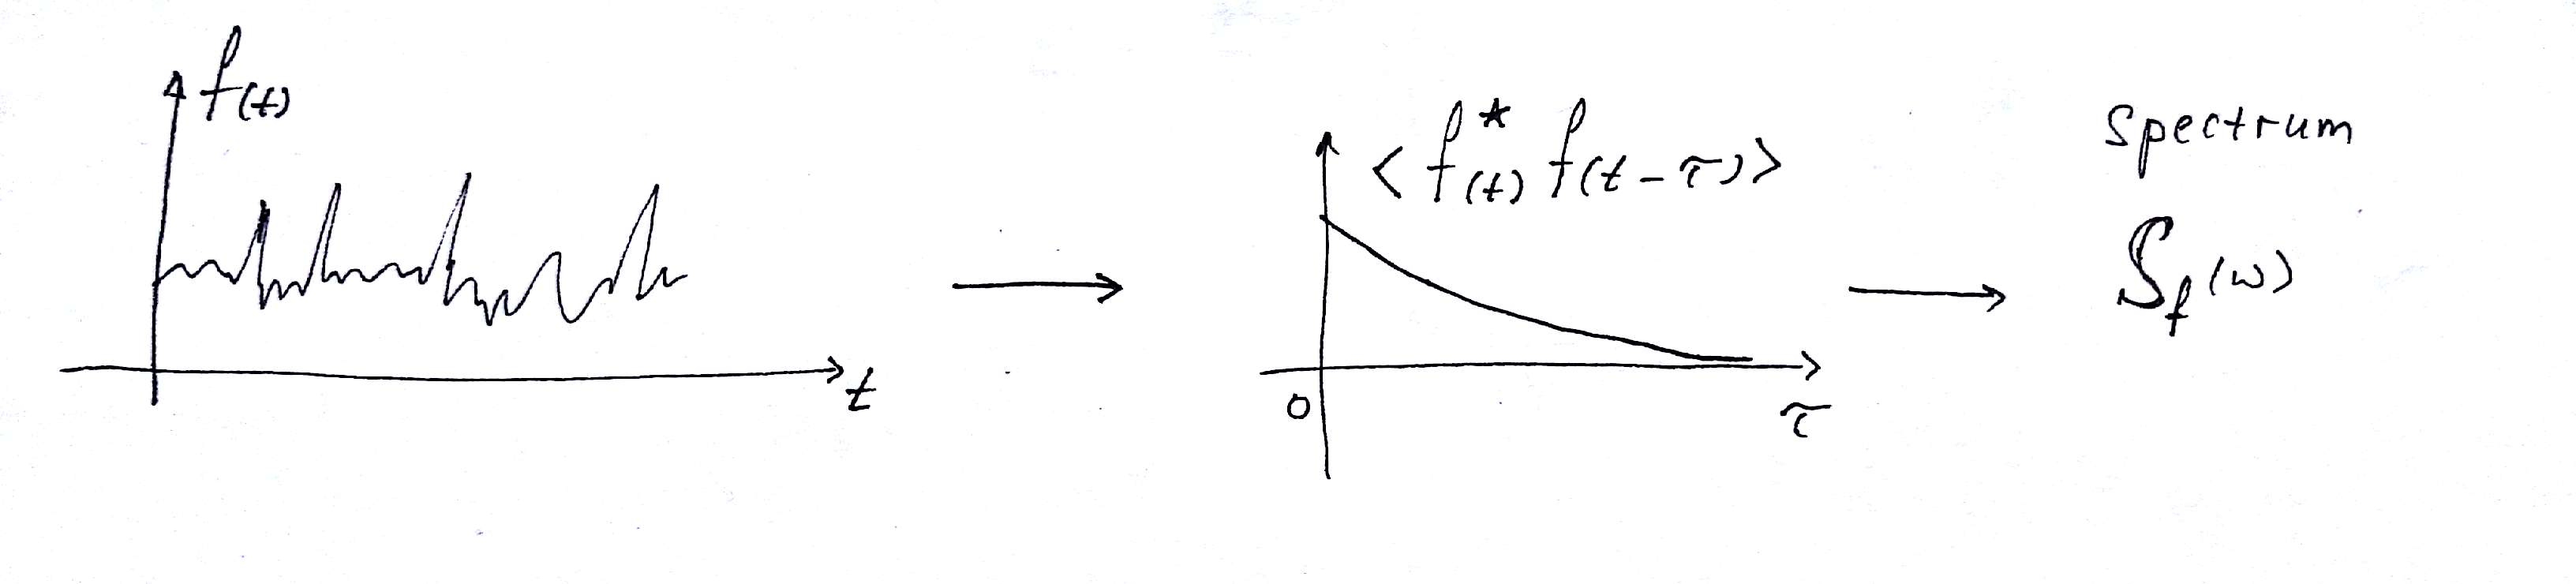
\includegraphics[width=0.85\linewidth]{fig/L9/wiener}
	\caption{Wiener--Khintchine theorem in 40 seconds}
	\label{fig:wiener}
\end{figure}

In our case instead of $f(t)$ we have $ \hat{a}(t) = \hat{\tilde{a}}(t) e^{-i \omega t}$ which gives
\begin{equation}
	\av{\hat{a}^{\dagger}(t_0) \hat{a}(t_0 + \tau)} = \av{\hat{\tilde{a}}^{\dagger}(t_0) \hat{\tilde{a}}(t_0 + \tau)} e^{- i \omega \tau} = \av{n} e^{- \frac{\Gamma\tau}{2}} e^{-i\omega \tau},
\end{equation}
where $\av{n} \myeq  \av{\hat{\tilde{a}}^{\dagger}(t_0) \hat{\tilde{a}}(t_0)}$ is the mean number of photons at the initial time $t_0$. Then the spectrum
\begin{equation}
	S(\nu) = \frac{1}{\pi} \av{n}  \int \limits_{-\infty}^{\infty} d \tau e^{-i \nu \tau} \cdot e^{- \frac{\Gamma\tau}{2}} e^{-i\omega \tau} = \frac{1}{\pi} \av{n} \frac{\Gamma/2}{\left( \nu - \omega \right)^2 + \left(\Gamma/2\right)^2}.
\end{equation}
This is a Lorentzian distribution centered at $\nu = \omega$ with a half--width $\Gamma$ (fig. \ref{fig:loren}). The quality factor is connected with our results and can be written as $Q = \frac{\omega}{\Gamma}$.

\begin{figure}[h!]
	\centering
	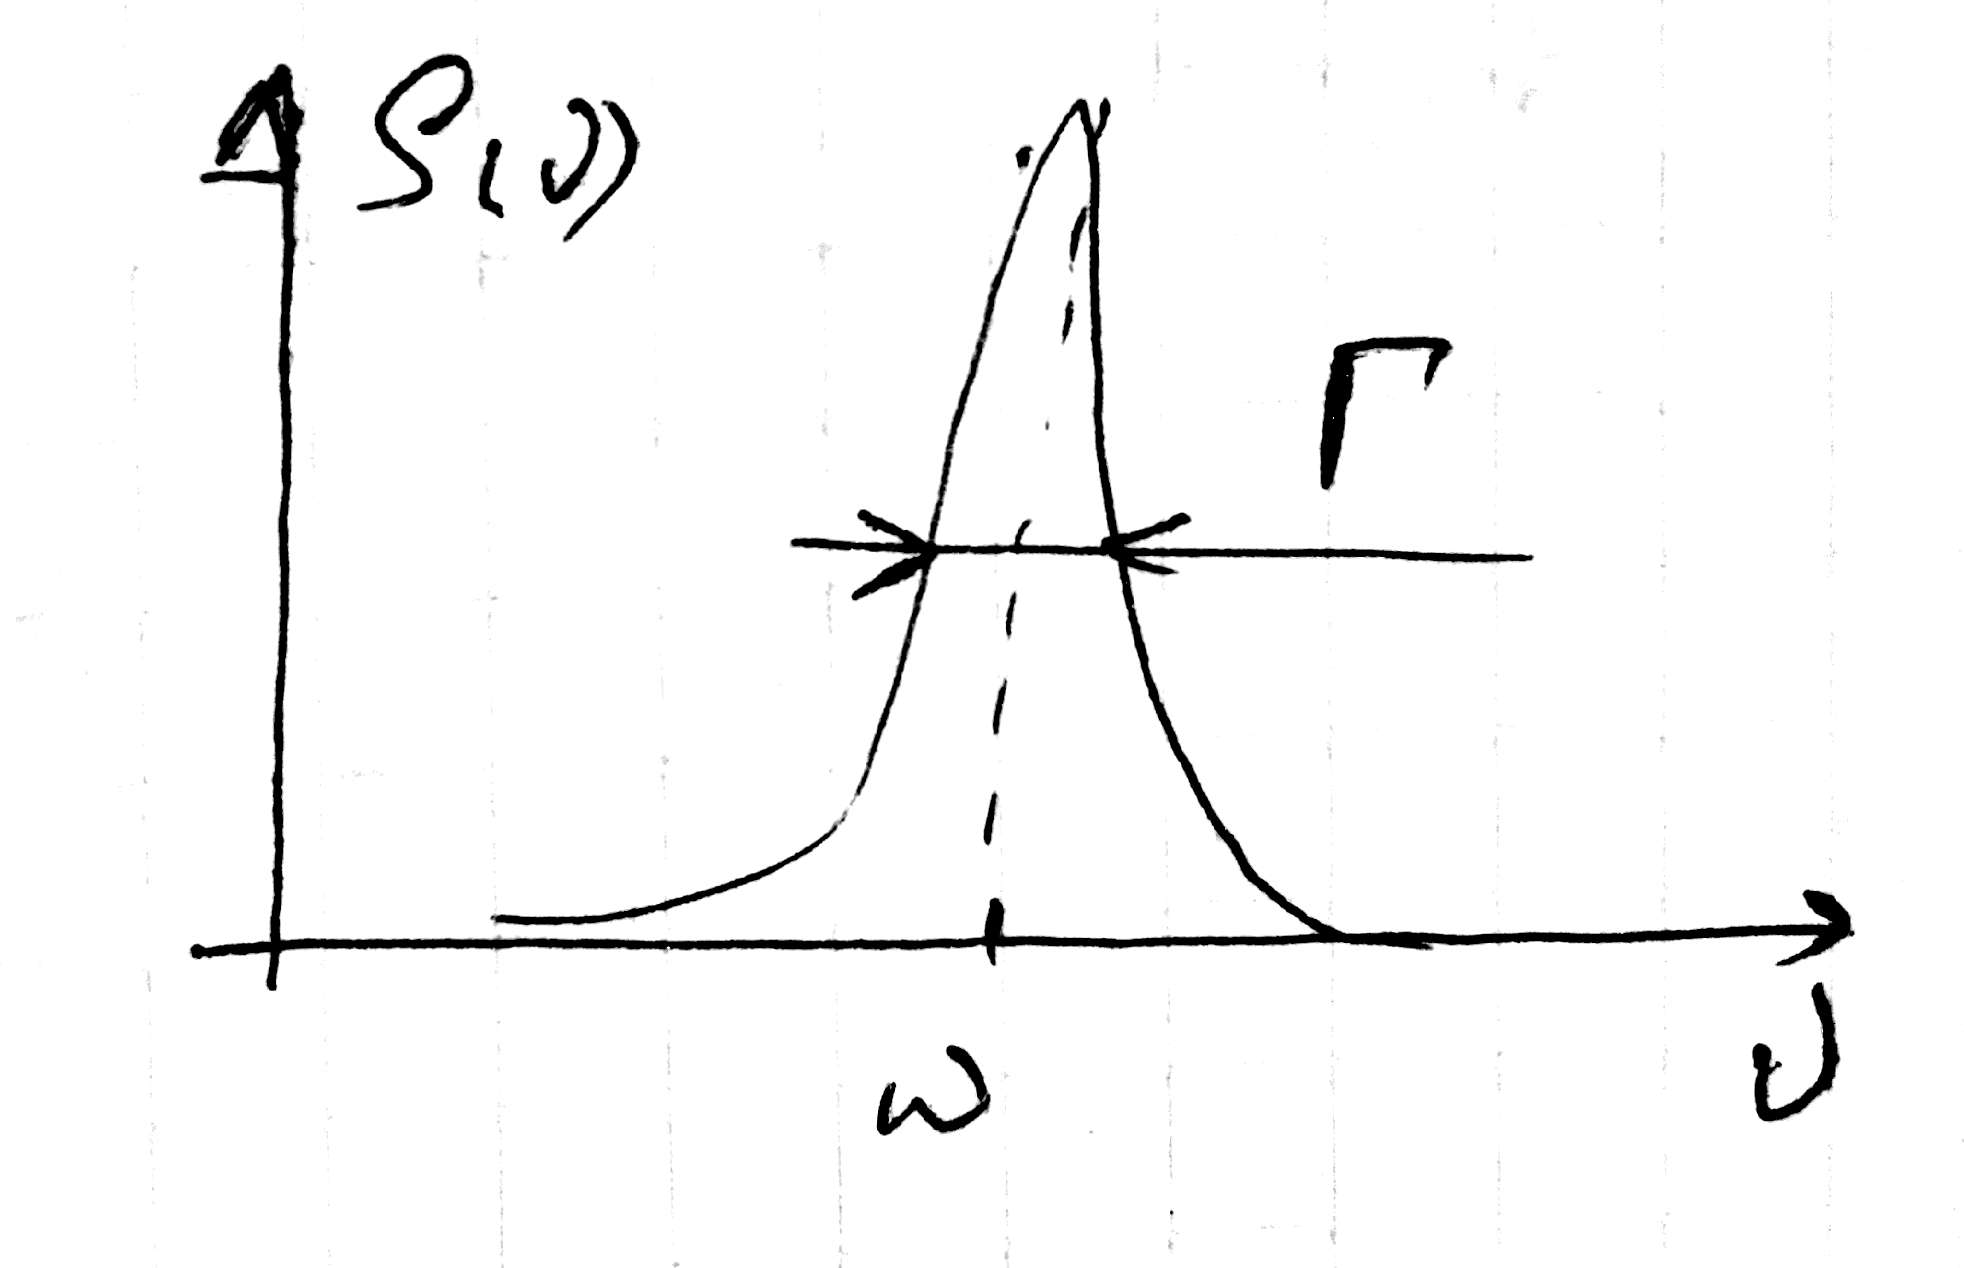
\includegraphics[width=0.4\linewidth]{fig/L9/L_1}
	\caption{Spectrum has a Lorentzian distribution shape}
	\label{fig:loren}
\end{figure}
